\section{Versuchsaufbau und Durchf\"uhrung}

\begin{figure}[hp]
    \centering
    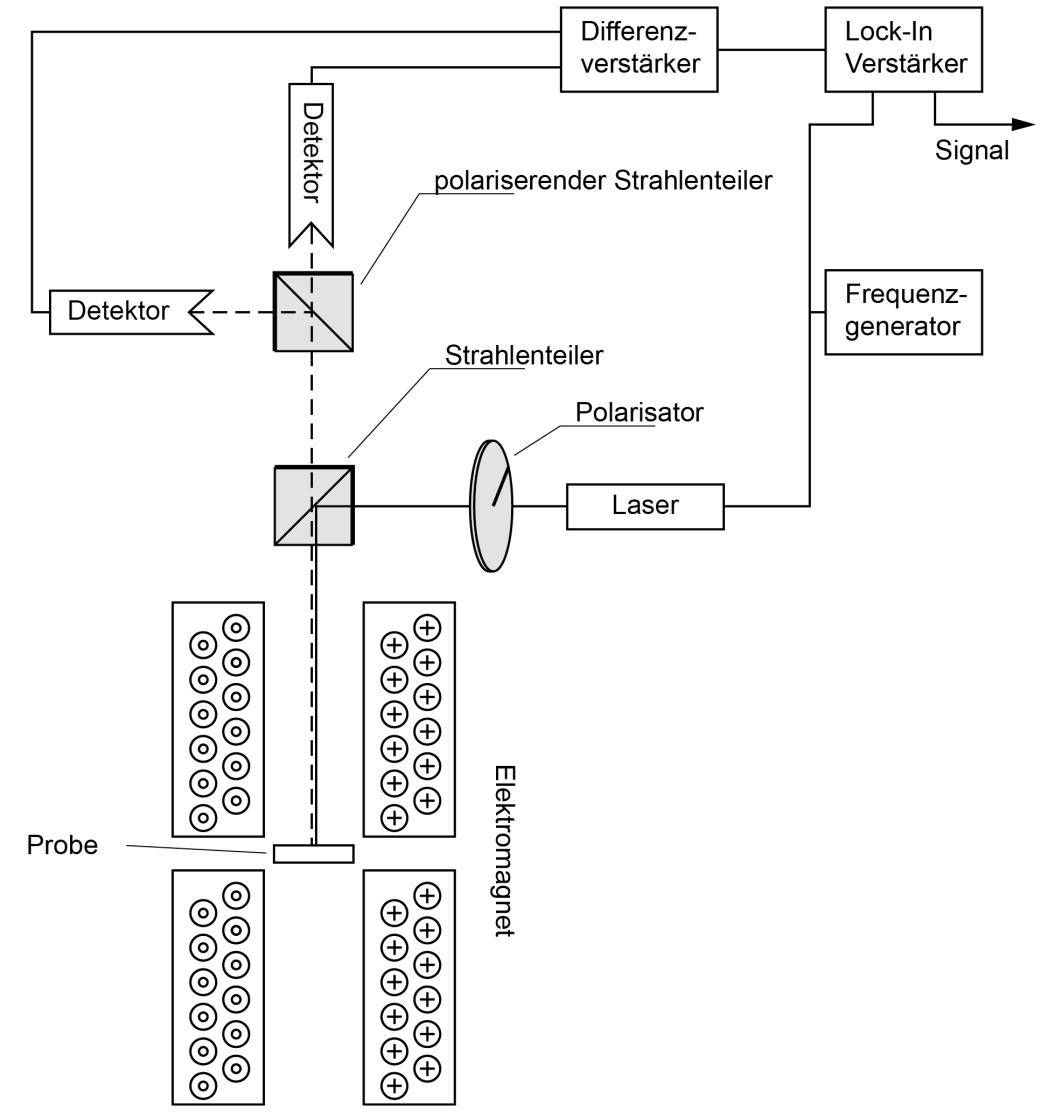
\includegraphics[width=1\textwidth]{../images/aufbau.png}
    \caption{
        Schematische Darstellung des Versuchaufbaus.
        Die Probe, eine magnetooptische Speicherdisc (MO), befindet sich in einer Spule, in der ein Magnetfeld erzeugt werden kann.
        Mit einem Laser wird durch einen Polarisator auf die Probe geschossen, wo dieser reflektiert wird und, abh"angig von der lokalen Magnetisierung, um den Kerrwinkel in der Polarisation gedreht wird.
        Der reflektierte Strahl wird am polarisierenden Strahlteiler in zwei orthogonale Polarisationen aufgeteilt, welche von separaten Detektoren erfasst werden.
        Die erzeugten Signale werden durch einen Differenzverst"arker verst"arkt und in einen Lock-In Verstarker geleitet.
        Dieser wirkt als schmalbandiger Filter, der nur die Frequenz durchl"asst, mit der der Laser, "uber den Frequenzgenerator, moduliert ist.
        Dies ist n"otig um das Rausche zu filtern, das durch den Differenzverst"arker mit verst"arkt wird.
        Das Signal aus dem Lock-In Verst"arker wird an einem Computer ausgelesen.
        Der Polarisator sollte etwa so eingestellt sein, dass die beiden Detektoren etwa gleich starke Signale empfangen, wodurch das Verh"altnis von Signal"anderung zu Signal maximiert wird.
        }
    \label{fig:aufbau}
\end{figure}

\subsection{Kalibrierung der Magnetfeldmessung}
Die Spule wird mit einer bekannten Spannung betrieben.
Um den Zusammenhang dieser Spannung mit der erzeugten Magnetfeldst"arke zu bestimmen wird zun"achst das Magnetfeld f"ur mehrere Spannung mit einer Hall-Sonde anstelle der Probe in Abbildung \vref{fig:aufbau} gemessen.
Die Spannung kann dabei am Computer durchgefahren, und die Kurve aufgenommen werden.

\subsection{Temperaturabh"angigkeit der Hysteresekurve}
In der eigentlichen Messung wird die Hysteresekurve f"ur verschiedene Temperaturen aufgenommen.
Zun"achst wird die Hall-Sonde wieder entfernt, da diese nicht f"ur h"ohere Temperaturen verwendet werden darf.
Anschlie{\ss}end wird die MO als Probe eingebracht.
Der Versuchsaufbau ist in Abbildung \ref{fig:aufbau} geschildert.
Um die Hysteresekurve aufzunehmen wird die Spannung, die die Spule treibt, kontinuierlich von 0 zum Maximum, dann zum Minimum und wieder zu 0 durchgefahren.
Dies wird am Computer erledigt, und auch die resultierende Signalspannung wird am Computer direkt aufgetragen.
Die Kalibrierungskurve wird vom Programm verwendet um die Spulen-Spannung direkt in eine Magnetfeldst"arke umzurechnen.
Aus der Hysteresekurve kann die Koerzitivfeldst"arke, also die zur Ummagnetisierung n"otige Feldst"arke direkt abgelesen werden.
Sie entspricht der halben Breite der Hysteresekurve.

Der Kerr-Winkel kann ebenfalls abgelesen werden.
F"ur eine total in eine Richtung Magnetisierte MO ist die Signalst"arke maximal oder minimal.
Die halbe Differenz zwischen maximaler und minimaler Signalst"arke kann also zu einem Kerr-Winkel umgerechnet werden.
Hierf"ur ist es n"otig, zu wissen, um wie stark sich die Signalspannung bei einer Drehung der Polarisation um einen bestimmten Winkel "andert.
Dies kann ermittelt werden, indem man den Polarisationsfilter mithilfe einer Mikrometerschraube fein verstellt und auf die "Anderung des Signals achtet.
Es ist entscheidend, danach die Differenz-Verst"arkung entweder nicht mehr zu "andern, oder eine "Anderung mit dem Signal zu verrechnen.

Die Messung der Hysterese kann nun f"ur verschiedene Temperaturen durchgef"uhrt werden, indem die MO in der Spule aufgeheizt wird.
Dies geschieht manuell, indem die Eingangsspannung der Heizung variiert wird.
Ein Thermometer zeigt die Aktuelle Temperatur an.
